% %% file: template.tex = LaTeX template for article-like report 
%% init: sometime 1993
%% last: Feb  8 2015  Rob Rutten  Deil
%% site: http://www.staff.science.uu.nl/~rutte101/rrweb/rjr-edu/manuals/student-report/

%% First read ``latex-bibtex-simple-manual.txt'' at
%% http://www.staff.science.uu.nl/~rutte101/Report_recipe.html

%% Start your report production by copying this file into your XXXX.tex.
%% Small changes to the header part will make it an A&A or ApJ manuscript.

%%%%%%%%%%%%%%%%%%%%%%%%%%%%%%%%%%%%%%%%%%%%%%%%%%%%%%%%%%%%%%%%%%%%%%%%%%%%
%\documentclass{aa}   %% Astronomy & Astrophysics style class
\documentclass[a4paper]{report}
\usepackage[inner=2cm,outer=2cm]{geometry}
%\geometry{a4paper}
\usepackage{graphicx,url,twoopt}
\usepackage{subcaption}
\usepackage{enumitem}
\usepackage{amsmath}
\usepackage[varg]{txfonts}           %% A&A font choice
%\usepackage{hyperref}                %% for pdflatex
%%\usepackage[breaklinks]{hyperref}  %% for latex+dvips
%%\usepackage{breakurl}              %% for latex+dvips
%\usepackage{pdfcomment}              %% for popup acronym meanings
%\usepackage{acronym}                 %% for popup acronym meanings
\usepackage{calrsfs}
\DeclareMathAlphabet{\pazocal}{OMS}{zplm}{m}{n}

\usepackage{natbib}
% \hypersetup{
%   colorlinks=true,   %% links colored instead of frames
%   urlcolor=blue,     %% external hyperlinks
%   linkcolor=red,     %% internal latex links (eg Fig)
% }

 %\bibpunct{(}{)}{;}{a}{}{,}    %% natbib cite format used by A&A and ApJ
 
%\pagestyle{plain}   %% undo the fancy A&A pagestyle 


%%%%%%%%%%%%%%%%%%%%%%%%%%%%%%%%%%%%%%%%%%%%%%%%%%%%%%%%%%%%%%%%%%%%%%%%%%%%
\begin{document}  

%\twocolumn[]
%\onecolumn
%%%%%%%%%%%%%%%%%%%%%%%%%%%%%%%%%%%%%%%%%%%%%%%%%%%%%%%%%%%%%%%%%%%%%%%%%%%%
\section{Introduction}\label{sec:introduction}
%%%%%%%%%%%%%%%%%%%%%%%%%%%%%%%%%%%%%%%%%%%%%%%%%%%%%%%%%%%%%%%%%%%%%%%%%%%%
In this project I am following the algorithm presented in Callin (2005)[1] for simulating the cosmic microwave background.  
This is the final part of the project.

In the first part I set up the background cosmology of the universe, and made a function that could find the conformal time as a function of $x$. 

In the second part I computed the electron fraction, electron density, optical depth and visibility function for times around and during recombination. 

The third part use the two previous to compute the density perturbations, and velocities of dark matter and baryons. This also included the temperature multi poles $\Theta_l$.

This final part combines all of these quantities to compute the final CMB power spectrum.

%%%%%%%%%%%%%%%%%%%%%%%%%%%%%%%%%%%%%%%%%%%%%%%%%%%%%%%%%%%%%%%%%%%%%%%%%%%%
\section{Equations}\label{sec:Equations}
%%%%%%%%%%%%%%%%%%%%%%%%%%%%%%%%%%%%%%%%%%%%%%%%%%%%%%%%%%%%%%%%%%%%%%%%%%%%
In this final part of the project we finally combine everything from the previous projects into the final CMB power spectrum. This is done by a few equations, the first of which is the Transfer function defined
\begin{equation}
 \Theta_l(k,x=0)=\int^0_{-\infty} \tilde{S}(k,x)j_l[k(\eta_0-\eta)]dx,
\end{equation}
where $j_l$ is the spherical Bessel functions, and S is the source function defined
\begin{equation}
 \tilde{S}(k,x) = \tilde{g}\bigg[\Theta_0+\Psi+\frac{1}{4}\Pi\bigg]+e^{-\tau}[\Psi^\prime-\Phi^\prime]-\frac{1}{ck}\frac{d}{dx}(\pazocal{H}\tilde{g}v_b) +\frac{3}{4c^2k^2}\frac{d}{dx}\bigg[\pazocal{H}\frac{d}{dx}(\pazocal
{H}\tilde{g}\Pi) \bigg].
\end{equation}
The only variable not explained earlier in this equation is $\Pi = \Theta_2 +\Theta_0^P+\Theta_2^P$, which contain two not previously used variables $\Theta_0^P$, and $\Theta_2^P$. These two are related to the polarization of the temperature multi poles. Since we chose to not include polarization and neutrinos in the last part of the project, these two can be set to zero, which means that for our case $\Pi = \Theta_2$.

The Source function deserves a bit of explaining. Its job is, as expected from its name, to source the spectrum for all $k$ modes at all $x$ values. It consist of four distinct terms each describing different effects. 

The first is the local monopole weighted by the visibility function $\tilde{g}$, this term also includes the fact that the photons climb out of a gravitational potential $\Psi$ and a small correction term $\Pi$. This redshifting of the photons is known as the Sachs-Wolfe effect. 

The second term is the integrated Sachs-Wolfe effect. This term takes care of the change due to changing gravitational fields the photons encounter on their way from the last scattering surface to us today.

The third term corrects for the Doppler effect, and the fourth term is still unaccounted for at the time of writing.


This is then multiplied by the spherical Bessel functions which projects this three dimensional field onto the surface of a sphere. This gives us the so-called Transfer function. Note however that this only takes care of the $x$ values. We still need to account for all $k$ modes, and all directions. And furthermore we have not yet included the spectrum left over by inflation which is what we started out with. (This is fine as was discussed previously since we use linearized equations.)

The full CMB power spectrum then reads 
\begin{equation}
 C_l = \int\frac{d^3k}{(2\pi)^3}P(k)\Theta_l^2(k)
\end{equation}
Here we finally scale by $P(k)$. Recall that we set $\Phi = 1$ as the initial condition, instead of $\Phi = P(k)$. This is fine since we are working with linearized equations. If the reader wants to use higher order equations this needs to be taken into account from the beginning.

Furthermore, if we consider that most inflationary models predict a Harrrison-Zel'dovich spectrum where 
\begin{equation}
 \frac{k^3}{2\pi^2}P(k) = \bigg(\frac{ck}{H_0}\bigg)^{n-1}
\end{equation}
holds, we can write the CMB power spectrum as
\begin{equation}
  C_l = \int_0^\infty\bigg(\frac{ck}{H_0}\bigg)^{n_s-1}\Theta_l^2(k)\frac{dk}{k}.
\end{equation}
Here $n_s$ is the spectral index, which according to the latest data from Planck[2] is $n_s = 0.968\pm0.006$.
Since the overall trend of the power spectrum is to drop as $l^{-2}$, it is a good idea to plot the spectrum in units of $l(l+1)/2\pi$ in $\mu K^2$. This makes it easier to see features in it. So far we have not normalized the spectrum in any way. Since we want to compare it to the observed spectrum, we simply normalize the spectrum to the maximum in our computed spectrum, and then multiply by the maximum in the Planck data. (This means that our spectrum may be scaled down or up compared to the observed one without us seeing it, which means we can only measure the form of our spectrum.)

With this we should now get a power spectrum that can be fitted to the data, making it possible to estimate the density components of the universe.

%%%%%%%%%%%%%%%%%%%%%%%%%%%%%%%%%%%%%%%%%%%%%%%%%%%%%%%%%%%%%%%%%%%%%%%%%%%%
\section{Implementation}\label{sec:Imp}
%%%%%%%%%%%%%%%%%%%%%%%%%%%%%%%%%%%%%%%%%%%%%%%%%%%%%%%%%%%%%%%%%%%%%%%%%%%%
From the earlier projects we have arrays with $x$, and $k$ values. We use these to calculate the source function. The result is then splined onto a high resolution grid in $x$ and $k$. We also see in the Transfer function that we want values for $j_l$ for a combination of $k$ and $\eta(x)$ values. It turns out that these numbers are in the range $[0,3400]$. Thus we sample $5400$ values linearly in this range, and then spline that so we can find arbitrary values in between them. 

We now have the spherical Bessel functions and Source functions for all values in our high resolution $k$ and $x$ grid making it possible to calculate the Transfer function. The $x$ and $k$ grids have $5000$ values in the same range as earlier, only this time the steps are linear through $x$, while $k$ is quadratic like before.

To find the Transfer function we need a numerical integration method. I have chosen to use the trapezoidal method. The integration limits go from $-\infty$ to $0$. Luckily for us the Source function is zero for almost all times except around the last scattering surface. Because of this we simply set the lower integration limit to a very low $x$ value still inside our grid.

The next step is to calculate $C_l$. This is done in precisely the same fashion. The only difference is the integration limits. We integrate over the $5000$ $k$ values in our grid. For information on why we only need this many k values for the integration see Callin(2005)[1]. In short it has to do with getting a good amount of values between each oscillation of the  Bessel function. 

%%%%%%%%%%%%%%%%%%%%%%%%%%%%%%%%%%%%%%%%%%%%%%%%%%%%%%%%%%%%%%%%%%%%%%%%%%%%
\section{Results}\label{sec:results}
%%%%%%%%%%%%%%%%%%%%%%%%%%%%%%%%%%%%%%%%%%%%%%%%%%%%%%%%%%%%%%%%%%%%%%%%%%%%
I have plotted various quantities while making this program to make sure that the various functions return sensible values.
An example is the integrand in the Transfer function (figure \ref{fig:integrand}). In the figure the source function gives a spike around recombination, while the Bessel function makes it oscillate at late times. There is no sign of anything wrong so far.

We should also make sure that the integrand in the power spectrum integral behaves appropriately. This can be seen in figure \ref{fig:integ}. Finally, the CMB power spectrum can be seen in figure \ref{fig:Cl}.

\begin{figure}[H]
 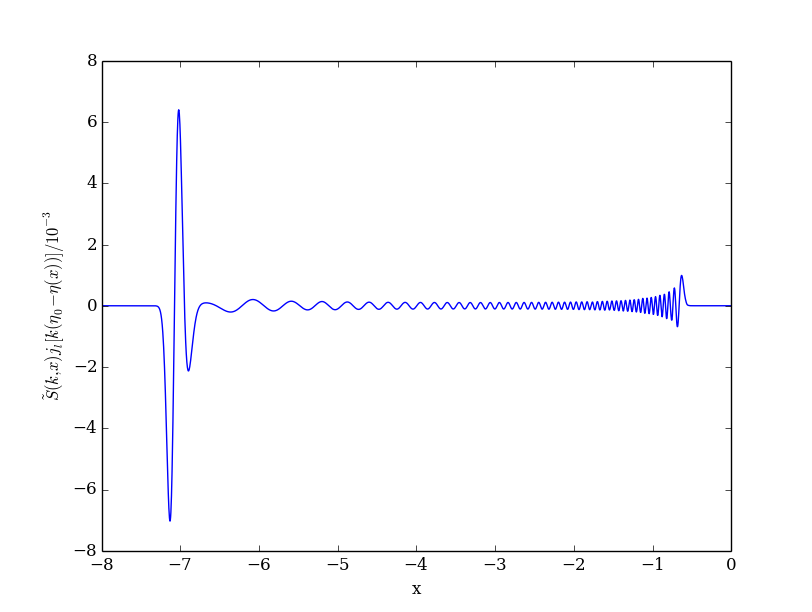
\includegraphics[width=\textwidth]{integrand.png}
 \caption{The integrand in the Transfer function integral for $l= 100$, and $k \approx160H_0/c$.}
 \label{fig:integrand}
\end{figure}

\begin{figure}[ht]
 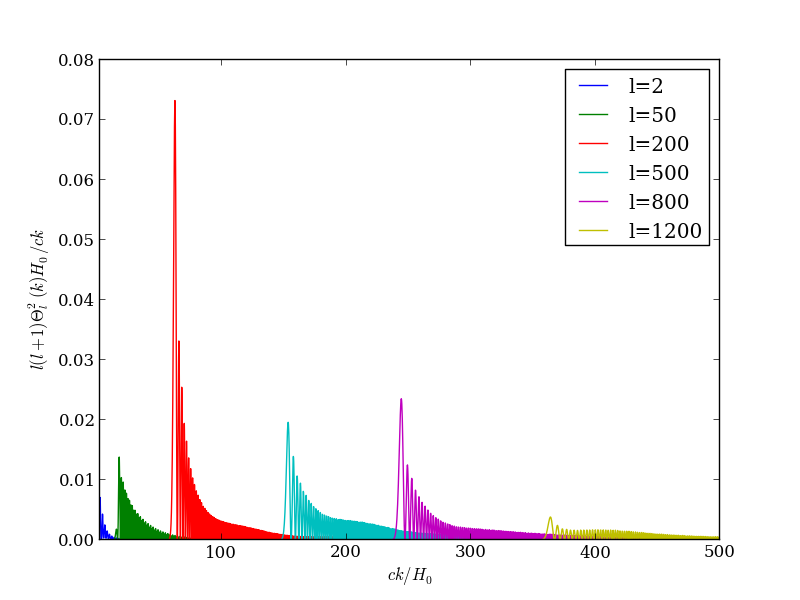
\includegraphics[width=\textwidth]{integ.png}
 \caption{The figure shows the integrand of the $C_l$ integral. We see that each $l$ gets its contribution from different ranges of $k$ values.}
 \label{fig:integ}
\end{figure}

\begin{figure}[ht]
 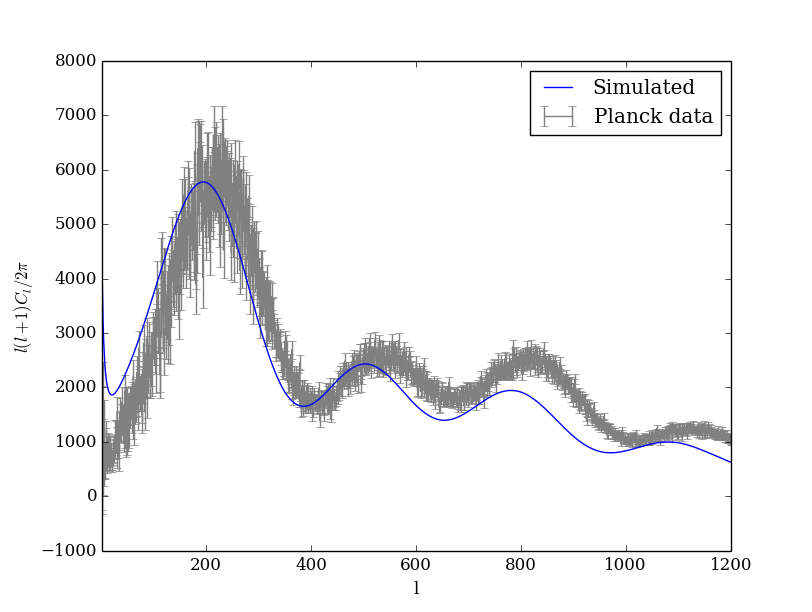
\includegraphics[width=\textwidth]{C_l_default.png}
 \caption{The CMB power spectrum. Computed in blue, and observed data in green. Something strange is happening for large scales in the computed spectrum. I assume this is a bug in my code. In reality the spectrum is low for small values of l.}
 \label{fig:Cl}
\end{figure}

%%%%%%%%%%%%%%%%%%%%%%%%%%%%%%%%%%%%%%%%%%%%%%%%%%%%%%%%%%%%%%%%%%%%%%%%%%%%
\section{Parameter estimation}\label{sec:param}
%%%%%%%%%%%%%%%%%%%%%%%%%%%%%%%%%%%%%%%%%%%%%%%%%%%%%%%%%%%%%%%%%%%%%%%%%%%%
Since we have a spectrum that resembles reality in some way we should try varying the cosmological parameters to see if we can make it match better. We start with varying $H_0$, or rather $h$ between $0.66$ and $0.74$, where the default value is $0.70$. This is shown in figure \ref{fig:hvary}
Let us change something else to see what that does to the spectrum. The next one is $\Omega_m$ between $0.20$ and $0.48$ which can be seen in figure \ref{fig:mvary}.
Since varying $h$ and $\Omega_m$ had such bizarre effects, we should also vary $\Omega_b$ to see what effect that has. This is shown in figure \ref{fig:mvary}. Clearly there is a bug in the program that makes the calculations unstable in some way. What is even stranger is that decreasing both $h$ and $\Omega_m$ returns the same bizarre power spectrum. This is probably a good place to start when trying to fix the program.

\begin{figure}[ht]
 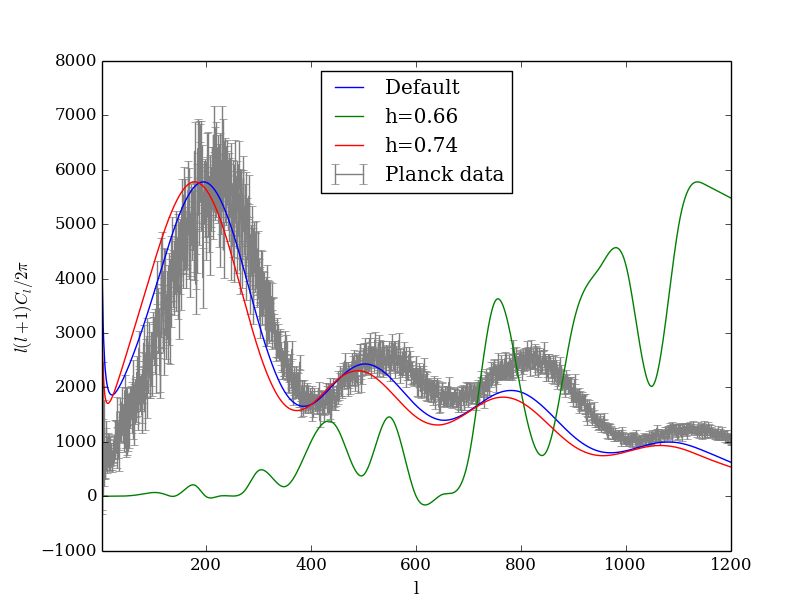
\includegraphics[width=\textwidth]{hvary.png}
 \caption{Varying $h$ proves to be catastrophic for the code. It is strange that increasing $h$ does very little, while decreasing it wrecks everything.}
 \label{fig:hvary}
\end{figure}


\begin{figure}[ht]
 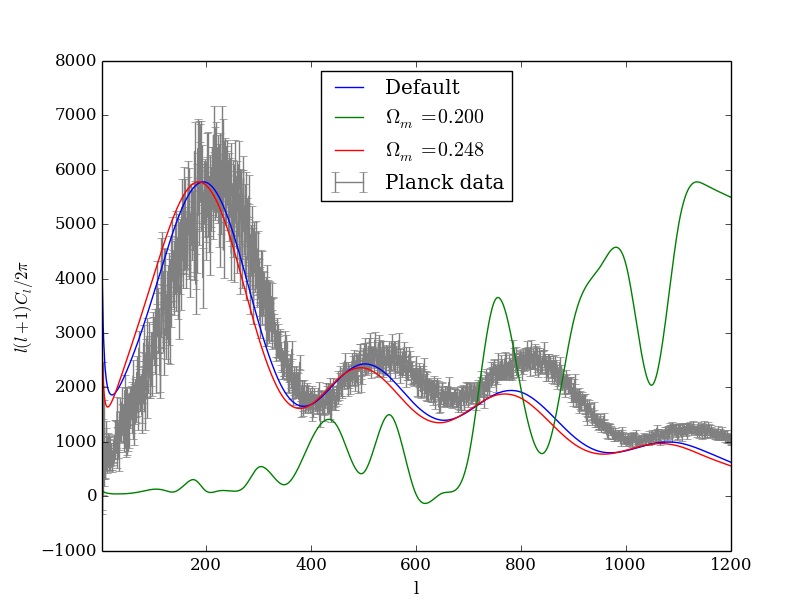
\includegraphics[width=\textwidth]{mvary.png}
 \caption{Here we see the same phenomenon appear again. Increasing the dark matter density shifts the spectrum to the left, and decreasing it returns the same spectrum as decreasing $h$ did.}
 \label{fig:mvary}
\end{figure}


\begin{figure}[ht]
 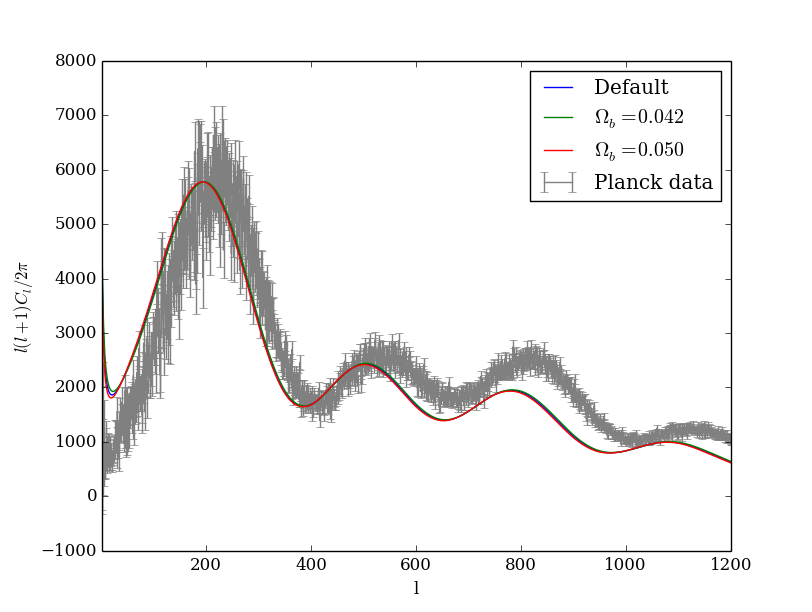
\includegraphics[width=\textwidth]{bvary.png}
 \caption{Strangely, varying $\Omega_b$ has almost no effect at all. One could argue that there is some change in the spectrum if one looks closely at the plot, but it should change much more than what we see here, so the bug is affecting this change as well.}
 \label{fig:bvary}
\end{figure}




%%%%%%%%%%%%%%%%%%%%%%%%%%%%%%%%%%%%%%%%%%%%%%%%%%%%%%%%%%%%%%%%%%%%%%%%%%%%
\section{Conclusion}\label{sec:Conc}
%%%%%%%%%%%%%%%%%%%%%%%%%%%%%%%%%%%%%%%%%%%%%%%%%%%%%%%%%%%%%%%%%%%%%%%%%%%%
We have seen that we can make a power spectrum that looks fairly close to the observed one even if we do not include neutrinos or polarization. There was however something strange happening in the power spectrum for low multi poles. 

It was also observed that changing $h$ resulted in a completely ridiculous spectrum, which is an obvious sign that something is wrong with the code. This bug was also present when varying $\Omega_m$, but strangely it was not visible when varying $\Omega_b$. However, we also saw that even if the bug did not destroy the spectrum when varying $\Omega_b$, the spectrum remained almost the same even though we changed something that should have changed the spectrum.

Since there is still a bug in the program that makes varying the parameters useless there was no point in making a Metropolis algorithm to estimate values of the various cosmological parameters. This is something I will have to do on my own time after fixing the bug. This is unfortunate as this would have been the icing on the cake for this project.


%%%%%%%%%%%%%%%%%%%%%%%%%%%%%%%%%%%%%%%%%%%%%%%%%%%%%%%%%%%%%%%%%%%%%%%%%%%%
\section{References}
%%%%%%%%%%%%%%%%%%%%%%%%%%%%%%%%%%%%%%%%%%%%%%%%%%%%%%%%%%%%%%%%%%%%%%%%%%%%
\begin{enumerate}[label= {[}\arabic*{]} ]
 \item P. Callin, astro-ph/0606683
 \item P. A. R. Ade et al. [Planck Collaboration], arXiv:1502.02114 [astro-ph.CO].
\end{enumerate}

\onecolumn 
%%%%%%%%%%%%%%%%%%%%%%%%%%%%%%%%%%%%%%%%%%%%%%%%%%%%%%%%%%%%%%%%%%%%%%%%%%%%
\section{Source code}\label{sec:files}
%%%%%%%%%%%%%%%%%%%%%%%%%%%%%%%%%%%%%%%%%%%%%%%%%%%%%%%%%%%%%%%%%%%%%%%%%%%%
The source code for the function made for computing the high resolution source function in evolution\_mod.f90 as well as the file cl\_mod.f90 file used for computing the final power spectrum is included for inspection. These files depend on all files previously used in the three earlier parts of the project.
\begin{verbatim}
module cl_mod
  use healpix_types
  use evolution_mod
  use sphbess_mod
  implicit none

  real(dp), allocatable, dimension(:,:) :: S, S2
  real(dp), allocatable, dimension(:)   :: x_hires, k_hires,cl_hires,l_hires
  real(dp), allocatable, dimension(:)   :: z_spline
  real(dp), allocatable, dimension(:,:) :: j_l,j_l2
  real(dp), allocatable, dimension(:)   :: integrand,besseltest
  real(dp),     allocatable, dimension(:,:)     :: Theta_l,integrand2
  integer(i4b), allocatable, dimension(:)       :: ls
contains
  ! Driver routine for (finally!) computing the CMB power spectrum
  subroutine compute_cls
    implicit none

    integer(i4b) :: i, j, l, l_num, x_num, n_spline
    real(dp)     :: S_func, j_func, z, eta, eta0, x0, x_min, x_max, d, e
    real(dp),     allocatable, dimension(:)       :: cls, cls2, ls_dp
    real(dp),     allocatable, dimension(:)       :: j_l_spline, j_l_spline2
    real(dp)                                      :: ax1,ax2,ak1,ak2,h1,h2,C_lint

    real(dp)           :: t1, t2, integral
    logical(lgt)       :: exist
    character(len=128) :: filename
    real(dp), allocatable, dimension(:) :: y, y2

    !precompute useful variables

    ! Set up which l's to compute
    l_num = 44
    allocate(ls(l_num))

    !test ls
    !ls = (/2,3,4,5,6/)
    
    ls = (/ 2, 3, 4, 6, 8, 10, 12, 15, 20, 30, 40, 50, 60, 70, 80, 90, 100, &
         & 120, 140, 160, 180, 200, 225, 250, 275, 300, 350, 400, 450, 500, 550, &
         & 600, 650, 700, 750, 800, 850, 900, 950, 1000, 1050, 1100, 1150, 1200 /)

    ! Task: Get source function from evolution_mod
    allocate(S(n_x_highres,n_k_highres))
    allocate(x_hires(n_x_highres),k_hires(n_k_highres))


    write(*,*) 'Compute hires Source function'
    call get_hires_source_function(x_hires, k_hires, S)
    
    !Test source func
    !write(*,*) 'S lores'
    !write(*,*) S_lores(301,50)
    !write(*,*) x_t(301),ks(50)
    !write(*,*) get_g(x_t(301)),Theta(301,0,50),Psi(301,50),Phi(301,50),Theta(301,2,50)

    !write(*,*) 'S hires'
    !write(*,*) S(1,1),S(n_x_highres,n_k_highres)


    !Test of x and k grid.
    !write(*,*) 'x_hires'
    !write(*,*) x_hires(1),x_hires(n_x_highres)
    !write(*,*) 'k_hires'
    !write(*,*) k_hires(1),k_hires(n_k_highres)

    


    ! Task: Initialize spherical Bessel functions for each l; use 5400 sampled points between 
    !       z = 0 and 3500. Each function must be properly splined
    n_spline = 5400
    allocate(z_spline(n_spline))    ! Note: z is *not* redshift, but simply the dummy argument
                                    ! of j_l(z)

    do i=1,n_spline
        z_spline(i) = 0.d0 + (i-1)*(3400.d0-0.d0)/(n_spline-1.d0)
    end do 

    !Test z_spline
    !write(*,*) 'z_spline'
    !write(*,*) z_spline(1), z_spline(n_spline)


    allocate(j_l(n_spline,l_num))
    allocate(j_l2(n_spline,l_num))



    !Calculate spherical bessel functions for select ls
    write(*,*) 'Compute spherical Bessel functions'
    do i =1,n_spline
        do l=1,l_num
            if(z_spline(i) > 2.d0) then
                call sphbes(ls(l),z_spline(i), j_l(i,l))
            endif
        end do
    end do

    !Spline across z for each l
    write(*,*) 'splining bessel'
    do l=1,l_num
          call spline(z_spline, j_l(:,l), yp1, ypn, j_l2(:,l))
    end do


    !Bessel test
    allocate(besseltest(n_x_highres))
    do i =1,n_x_highres 
        besseltest(i) =  j_lfunc(17,k_hires(2000),x_hires(i))
    end do

    open (unit=34 ,file="besseltest.dat",action="write",status="replace")
    do i=1,n_x_highres
        write (34 ,*) besseltest(i)
    end do 
    close (34)

    ! Overall task: Compute the C_l's for each given l

    !Compute the transfer function, Theta_l(k)
    ! For this I use trapezoidal intergration. Better methods should be implemented
    ! for better precision.
    write(*,*) 'Starting integration of Theta_l'
    allocate(Theta_l(l_num,n_k_highres))
    allocate(integrand(n_x_highres))
    allocate(integrand2(l_num,n_k_highres))
    allocate(cls(l_num))
    allocate(cls2(l_num))

    open (unit=123, file="integrand1.dat", action="write", status="replace")
    open (unit=124, file="integrand2.dat", action="write", status="replace")
    open (unit=125, file="integrand3.dat", action="write", status="replace")
    open (unit=126, file="integrand4.dat", action="write", status="replace")
    open (unit=127, file="integrand5.dat", action="write", status="replace")
    open (unit=128, file="integrand6.dat", action="write", status="replace")


    do l =1,l_num
        write(*,*)'l =',ls(l)

        !write(*,*) 'Doing theta_l integration'
        do k=1,n_k_highres
            !write(*,*)'k = ',k
            !trapezoidal method start
            ax1 = x_hires(1)
            ax2 = x_hires(n_x_highres)
            h1 = (ax2-ax1)/n_x_highres

            !write(*,*) 'Before integrand part'
            do i=1,n_x_highres
                integrand(i) = S(i,k)*j_lfunc(l,k_hires(k),x_hires(i))
            end do

            if(l==17 .and. k==2000) then
                write(*,*)'writing integrand to file for l=17,k=2000'
                open (unit=17 ,file="Sj_l.dat",action="write",status="replace")
                    do i=1,n_x_highres
                        write (17 ,*) integrand(i)
                    end do 
                close (17)
            !stop
            end if
            !write(*,*) 'before trapezoidal part'
            Theta_l(l,k) = 0.5d0*(integrand(1)+integrand(n_x_highres))
            do i=2,n_x_highres-1
                Theta_l(l,k) = Theta_l(l,k) +integrand(i)
            end do
            Theta_l(l,k) = h1*Theta_l(l,k)
            !write(*,*) 'after trapezoidal part'
        end do
        !write(*,*) 'After theta_l integration'
        !trapezoidal method end

        !Integrate P(k) * (Theta_l^2 / k) over k to find un-normalized C_l's
        !trapezoidal method start
        !write(*,*)'doing c_l integration'

        ak1 = k_hires(1)
        ak2 = k_hires(n_k_highres)
        h2 = (ak2-ak1)/n_k_highres

        do k=1,n_k_highres
            integrand2(l,k) = (c*k_hires(k)/H_0)**(n_s-1.d0)*Theta_l(l,k)**2/k_hires(k)
        end do


        !write the integrand in cl integral to file
        if(ls(l)==2) then
            do k=1,n_k_highres
                write (123,'(*(2X, ES14.6E3))') c*k_hires(k)/H_0 , ls(l)*(ls(l)+1.d0)*&
                      Theta_l(l,k)**2/(c*k_hires(k)/H_0)
            end do
        end if 
        if(ls(l)==50) then
            do k=1,n_k_highres
                write (124,'(*(2X, ES14.6E3))') ls(l)*(ls(l)+1.d0)*Theta_l(l,k)**2 &
                      /(c*k_hires(k)/H_0)
            end do
        end if 
        if(ls(l)==200) then
            do k=1,n_k_highres
                write (125,'(*(2X, ES14.6E3))') ls(l)*(ls(l)+1.d0)*Theta_l(l,k)**2 &
                      /(c*k_hires(k)/H_0)
            end do
        end if 
        if(ls(l)==500) then
            do k=1,n_k_highres
                write (126,'(*(2X, ES14.6E3))') ls(l)*(ls(l)+1.d0)*Theta_l(l,k)**2 &
                      /(c*k_hires(k)/H_0)
            end do
        end if 
        if(ls(l)==800) then
            do k=1,n_k_highres
                write (127,'(*(2X, ES14.6E3))') ls(l)*(ls(l)+1.d0)*Theta_l(l,k)**2 &
                      /(c*k_hires(k)/H_0)
            end do
        end if 
        if(ls(l)==1200) then
            do k=1,n_k_highres
                write (128,'(*(2X, ES14.6E3))') ls(l)*(ls(l)+1.d0)*Theta_l(l,k)**2 &
                      /(c*k_hires(k)/H_0)
            end do
        end if 



        C_lint = 0.5d0*(integrand2(l,1)+integrand2(l,n_k_highres))
        do k=2,n_k_highres-1
                !write(*,*) 'k=',k
                C_lint = C_lint + integrand2(l,k)
        end do

        !Store C_l in an array.
        cls(l) = h2*C_lint *ls(l)*(ls(l)+1.d0)/(2.d0*pi)
        !trapezoidal method end
    end do

    close(123)
    close(124)
    close(125)
    close(126)
    close(127)
    close(128)

    !This is needed to make the spline funciton happy(it demands double precision)
    write(*,*) 'converting ls to double precision'
    allocate(ls_dp(l_num))
    do l=1,l_num
        ls_dp(l) = ls(l)
    end do

    !Spline C_l's found above, and output smooth C_l curve for each integer l
    write(*,*)'splining cls'
    call spline(ls_dp, cls, yp1, ypn, cls2)
    write(*,*)'done splining cls'

    allocate(l_hires(int(maxval(ls))))
    allocate(cl_hires(int(maxval(ls))))

    write(*,*) 'making l_hires'
    do l=1,int(maxval(ls))
        l_hires(l) = l
    end do

    !Find Cls for all ls, also those not in the original list

    write(*,*)'saving splined cls'
    do l=1,int(maxval(ls))
        cl_hires(l) = splint(ls_dp, cls, cls2, l_hires(l))
    end do

  end subroutine compute_cls
  
  function j_lfunc(l,k,x)
      implicit none
      integer(i4b),intent(in) :: l
      real(dp), intent(in)    :: x,k
      real(dp)                :: j_lfunc
      !write(*,*)'inside j_lfunc'
      j_lfunc = splint(z_spline,j_l(:,l),j_l2(:,l),k*(get_eta(0.d0)-get_eta(x)))
      !write(*,*)'j_lfunc calculated'
  end function j_lfunc


end module cl_mod
\end{verbatim}
\newpage

\begin{verbatim}
  subroutine get_hires_source_function(x_hires, k_hires, S)
    implicit none

    real(dp), allocatable, dimension(:),   intent(out) :: x_hires, k_hires
    real(dp), allocatable, dimension(:,:), intent(out) :: S

    integer(i4b) :: i,k
    real(dp)     :: g, dg, ddg, dt, tau, ddt, Pi_c, dPi, ddPi,H_p,dH_p

    ! Task: Output a pre-computed 2D array (over k and x) for the 
    !       source function, S(k,x). Remember to set up (and allocate) output 
    !       k and x arrays too. 

    allocate(x_hires(n_x_highres),k_hires(n_k_highres))

    do i=1,n_x_highres    
        do k=1,n_k_highres
            x_hires(i) = x_init + (x_0-x_init)*(i-1.d0)/(n_x_highres-1.d0)
            k_hires(k) = k_min  + (k_max -k_min)*((k-1.d0)/(n_k_highres-1.d0))**2
        end do 
    end do

    !Test of x and k grid.
    !write(*,*) 'x_hires'
    !write(*,*) x_hires(1),x_hires(n_x_highres)
    !write(*,*) 'k_hires'
    !write(*,*) k_hires(1),k_hires(n_k_highres)
    !write(*,*) 'ks'
    !write(*,*) ks(1),ks(n_k)

    ! Substeps:
    !   1) First compute the source function over the existing k and x
    !      grids
    allocate(S_lores(1:n_t,1:n_k))
    allocate(S_coeff(4,4,n_t,n_k))

    allocate(S(n_x_highres,n_k_highres))

    do k=1,n_k
        k_current = ks(k)
        ck_current= c*k_current

        do i=1,n_t
            g     = get_g(x_t(i))
            dg    = get_dg(x_t(i))
            ddg   = get_ddg(x_t(i))
            tau   = get_tau(x_t(i))
            dt    = get_dtau(x_t(i))
            ddt   = get_ddtau(x_t(i))
            H_p   = get_H_p(x_t(i))
            dH_p  = get_dH_p(x_t(i))
            Pi_c    = Theta(i,2,k)
            dPi   = dTheta(i,2,k)

            ddPi  = 2.d0*ck_current/(5.d0*H_p)*(-dH_p/H_p*Theta(i,1,k) + dTheta(i,1,k)) &
                    +0.3d0*(ddt*Pi_c+dt*dPi) &
                    -3.d0*ck_current/(5.d0*H_p)*(-dH_p/H_p*Theta(i,3,k) + dTheta(i,3,k))

            S_lores(i,k) = g*(Theta(i,0,k) +Psi(i,k) + .25d0*Pi_c) &
                           +exp(-tau)*(dPsi(i,k)-dPhi(i,k)) &
                           -1.d0/ck_current*(H_p*(g*dv_b(i,k) + v_b(i,k)*dg) + g*v_b(i,k)*dH_p) &
                           +.75d0/ck_current**2*((H_0**2/2.d0*((Omega_m+Omega_b)/exp(x_t(i)) &
                           +4.d0*Omega_r/exp(2.d0*x_t(i)) +4.d0*Omega_lambda*exp(2.d0*x_t(i))))*&
                           g*Pi_c +3.d0*H_p*dH_p*(dg*Pi_c+g*dPi)+H_p**2* &
                           (ddg*Pi_c +2.d0*dg*dPi+g*ddPi))
        end do
    end do

    !2) Then spline this function with a 2D spline
    call splie2_full_precomp(x_t, ks, S_lores,S_coeff)

    !3) Finally, resample the source function on a high-resolution uniform
    !      5000 x 5000 grid and return this, together with corresponding
    !      high-resolution k and x arrays
    do k=1,n_k_highres
        do i=1,n_x_highres
            S(i,k) = splin2_full_precomp(x_t, ks, S_coeff, x_hires(i), k_hires(k))
        end do
    end do
  end subroutine get_hires_source_function

\end{verbatim}


%%%%%%%%%%%%%%%%%%%%%%%%%%%%%%%%%%%%%%%%%%%%%%%%%%%%%%%%%%%%%%%%%%%%%%%%%%%%
%\begin{acknowledgements}
%\end{acknowledgements}

\end{document}